\section{Teoremi Dispensa 7}

\subsection{Teorema a pag. 9}

Sia $\Gamma = \langle I_{\Gamma},\ S_{\Gamma},\ \pi_{\Gamma} \rangle$ un problema decisionale e sia $\chi: I_{\Gamma} \rightarrow \Sigma^*$
una sua codifica ragionevole, se $\chi(I_{\Gamma}) \in \textbf{P}$\footnote{Questo perché la decisione del linguaggio delle istanze
deve richiedere "poche risorse", altrimenti non sappiamo dire nulla riguardo il linguaggio del problema complemento.}, allora 
\[
L_{\Gamma}(\chi) \in \textbf{NP} \Rightarrow L_{\Gamma^c}(\chi) \in \textbf{coNP} 
\]

\paragraph*{Dimostrazione:}

\begin{itemize}
    \item []{
        Poiché $\chi(I_{\Gamma}) \in \textbf{P}$, allora $\exists,\ T,\ h \in \mathbb{N}$ tale che $\forall x \in \Sigma^*$
        $T(x) =
        \begin{cases} 
            & q_{A} \Leftrightarrow x\in \chi(I_{\Gamma})\\
            & q_{R} \Leftrightarrow x\notin \chi(I_{\Gamma})\\
        \end{cases}$ 
        $\land\ dtime(T, x) \leq |x|^h$.
    }
    \item []{
        Se $L_{\Gamma}(\chi) \in \textbf{NP}$ allora $\exists\ NT, k \in \mathbb{N}$ tale che 
        \[
            \forall x \in L_{\Gamma}(\chi)\ NT(x) = q_{A}\ \land\ \forall x \notin L_{\Gamma}(\chi)\ NT(x)
            \neq q_{A}\ \land\ ntime(NT, x) \leq |x|^k
        \] 
    }
    \end{itemize}
    
Da $T$ e $NT$ deriviamo $NT^{'}$ con input $x \in \Sigma^*$ che opera nel seguente modo:
\begin{itemize}
    \item [FASE 1: ] Simula $T(x)$. Se $T(x) = q_{R}$ allora $NT^{'} = q_{A}$. Se $T(x) = q_{A}$ allora esegui la fase 2.
    \item [FASE 2: ] Simula $NT(x)$.
\end{itemize}

Quindi $NT^{'}$ accetta se e soltanto se $x \in L_{\Gamma} \lor x \notin \chi(I_{\Gamma})$, ossia se e soltanto se $x \in (L_{\Gamma^c})^c$.
Dunque $NT^{'}$ accetta $L_{\Gamma^c}^c$, e $ntime(NT^{'}, x) \leq |x|^{\max(h, k)}$, quindi $(L_{\Gamma^c})^c \in \textbf{NP} \Rightarrow L_{\Gamma^c} \in \textbf{coNP}$.

\begin{figure}[h]
    \centering
    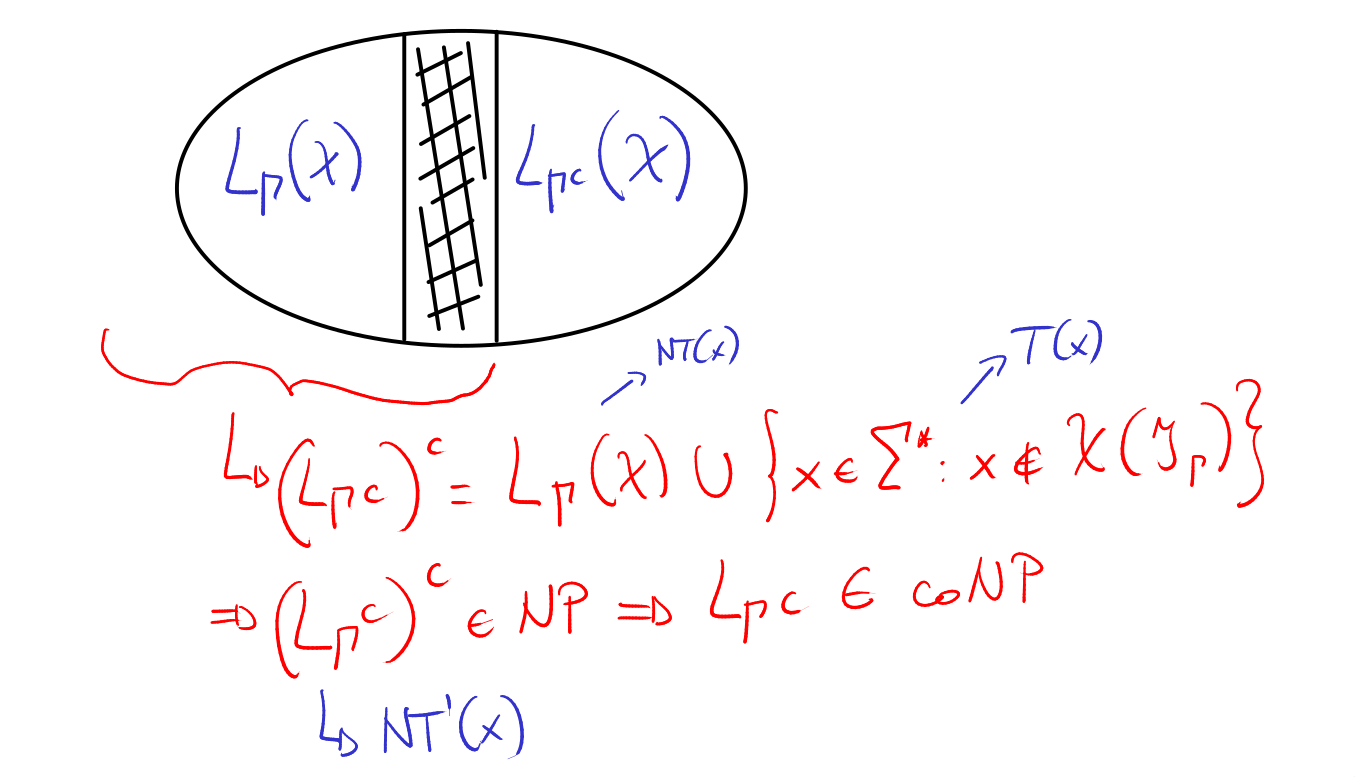
\includegraphics[width=0.8\textwidth]{../img/th7.png}
    \caption{Schema grafico della dimostrazione}
  \end{figure}